% Options for packages loaded elsewhere
\PassOptionsToPackage{unicode}{hyperref}
\PassOptionsToPackage{hyphens}{url}
%
\documentclass[
]{article}
\usepackage{amsmath,amssymb}
\usepackage{iftex}
\ifPDFTeX
  \usepackage[T1]{fontenc}
  \usepackage[utf8]{inputenc}
  \usepackage{textcomp} % provide euro and other symbols
\else % if luatex or xetex
  \usepackage{unicode-math} % this also loads fontspec
  \defaultfontfeatures{Scale=MatchLowercase}
  \defaultfontfeatures[\rmfamily]{Ligatures=TeX,Scale=1}
\fi
\usepackage{lmodern}
\ifPDFTeX\else
  % xetex/luatex font selection
\fi
% Use upquote if available, for straight quotes in verbatim environments
\IfFileExists{upquote.sty}{\usepackage{upquote}}{}
\IfFileExists{microtype.sty}{% use microtype if available
  \usepackage[]{microtype}
  \UseMicrotypeSet[protrusion]{basicmath} % disable protrusion for tt fonts
}{}
\makeatletter
\@ifundefined{KOMAClassName}{% if non-KOMA class
  \IfFileExists{parskip.sty}{%
    \usepackage{parskip}
  }{% else
    \setlength{\parindent}{0pt}
    \setlength{\parskip}{6pt plus 2pt minus 1pt}}
}{% if KOMA class
  \KOMAoptions{parskip=half}}
\makeatother
\usepackage{xcolor}
\usepackage[margin=1in]{geometry}
\usepackage{color}
\usepackage{fancyvrb}
\newcommand{\VerbBar}{|}
\newcommand{\VERB}{\Verb[commandchars=\\\{\}]}
\DefineVerbatimEnvironment{Highlighting}{Verbatim}{commandchars=\\\{\}}
% Add ',fontsize=\small' for more characters per line
\usepackage{framed}
\definecolor{shadecolor}{RGB}{248,248,248}
\newenvironment{Shaded}{\begin{snugshade}}{\end{snugshade}}
\newcommand{\AlertTok}[1]{\textcolor[rgb]{0.94,0.16,0.16}{#1}}
\newcommand{\AnnotationTok}[1]{\textcolor[rgb]{0.56,0.35,0.01}{\textbf{\textit{#1}}}}
\newcommand{\AttributeTok}[1]{\textcolor[rgb]{0.13,0.29,0.53}{#1}}
\newcommand{\BaseNTok}[1]{\textcolor[rgb]{0.00,0.00,0.81}{#1}}
\newcommand{\BuiltInTok}[1]{#1}
\newcommand{\CharTok}[1]{\textcolor[rgb]{0.31,0.60,0.02}{#1}}
\newcommand{\CommentTok}[1]{\textcolor[rgb]{0.56,0.35,0.01}{\textit{#1}}}
\newcommand{\CommentVarTok}[1]{\textcolor[rgb]{0.56,0.35,0.01}{\textbf{\textit{#1}}}}
\newcommand{\ConstantTok}[1]{\textcolor[rgb]{0.56,0.35,0.01}{#1}}
\newcommand{\ControlFlowTok}[1]{\textcolor[rgb]{0.13,0.29,0.53}{\textbf{#1}}}
\newcommand{\DataTypeTok}[1]{\textcolor[rgb]{0.13,0.29,0.53}{#1}}
\newcommand{\DecValTok}[1]{\textcolor[rgb]{0.00,0.00,0.81}{#1}}
\newcommand{\DocumentationTok}[1]{\textcolor[rgb]{0.56,0.35,0.01}{\textbf{\textit{#1}}}}
\newcommand{\ErrorTok}[1]{\textcolor[rgb]{0.64,0.00,0.00}{\textbf{#1}}}
\newcommand{\ExtensionTok}[1]{#1}
\newcommand{\FloatTok}[1]{\textcolor[rgb]{0.00,0.00,0.81}{#1}}
\newcommand{\FunctionTok}[1]{\textcolor[rgb]{0.13,0.29,0.53}{\textbf{#1}}}
\newcommand{\ImportTok}[1]{#1}
\newcommand{\InformationTok}[1]{\textcolor[rgb]{0.56,0.35,0.01}{\textbf{\textit{#1}}}}
\newcommand{\KeywordTok}[1]{\textcolor[rgb]{0.13,0.29,0.53}{\textbf{#1}}}
\newcommand{\NormalTok}[1]{#1}
\newcommand{\OperatorTok}[1]{\textcolor[rgb]{0.81,0.36,0.00}{\textbf{#1}}}
\newcommand{\OtherTok}[1]{\textcolor[rgb]{0.56,0.35,0.01}{#1}}
\newcommand{\PreprocessorTok}[1]{\textcolor[rgb]{0.56,0.35,0.01}{\textit{#1}}}
\newcommand{\RegionMarkerTok}[1]{#1}
\newcommand{\SpecialCharTok}[1]{\textcolor[rgb]{0.81,0.36,0.00}{\textbf{#1}}}
\newcommand{\SpecialStringTok}[1]{\textcolor[rgb]{0.31,0.60,0.02}{#1}}
\newcommand{\StringTok}[1]{\textcolor[rgb]{0.31,0.60,0.02}{#1}}
\newcommand{\VariableTok}[1]{\textcolor[rgb]{0.00,0.00,0.00}{#1}}
\newcommand{\VerbatimStringTok}[1]{\textcolor[rgb]{0.31,0.60,0.02}{#1}}
\newcommand{\WarningTok}[1]{\textcolor[rgb]{0.56,0.35,0.01}{\textbf{\textit{#1}}}}
\usepackage{longtable,booktabs,array}
\usepackage{calc} % for calculating minipage widths
% Correct order of tables after \paragraph or \subparagraph
\usepackage{etoolbox}
\makeatletter
\patchcmd\longtable{\par}{\if@noskipsec\mbox{}\fi\par}{}{}
\makeatother
% Allow footnotes in longtable head/foot
\IfFileExists{footnotehyper.sty}{\usepackage{footnotehyper}}{\usepackage{footnote}}
\makesavenoteenv{longtable}
\usepackage{graphicx}
\makeatletter
\def\maxwidth{\ifdim\Gin@nat@width>\linewidth\linewidth\else\Gin@nat@width\fi}
\def\maxheight{\ifdim\Gin@nat@height>\textheight\textheight\else\Gin@nat@height\fi}
\makeatother
% Scale images if necessary, so that they will not overflow the page
% margins by default, and it is still possible to overwrite the defaults
% using explicit options in \includegraphics[width, height, ...]{}
\setkeys{Gin}{width=\maxwidth,height=\maxheight,keepaspectratio}
% Set default figure placement to htbp
\makeatletter
\def\fps@figure{htbp}
\makeatother
\setlength{\emergencystretch}{3em} % prevent overfull lines
\providecommand{\tightlist}{%
  \setlength{\itemsep}{0pt}\setlength{\parskip}{0pt}}
\setcounter{secnumdepth}{5}
\newlength{\cslhangindent}
\setlength{\cslhangindent}{1.5em}
\newlength{\csllabelwidth}
\setlength{\csllabelwidth}{3em}
\newlength{\cslentryspacingunit} % times entry-spacing
\setlength{\cslentryspacingunit}{\parskip}
\newenvironment{CSLReferences}[2] % #1 hanging-ident, #2 entry spacing
 {% don't indent paragraphs
  \setlength{\parindent}{0pt}
  % turn on hanging indent if param 1 is 1
  \ifodd #1
  \let\oldpar\par
  \def\par{\hangindent=\cslhangindent\oldpar}
  \fi
  % set entry spacing
  \setlength{\parskip}{#2\cslentryspacingunit}
 }%
 {}
\usepackage{calc}
\newcommand{\CSLBlock}[1]{#1\hfill\break}
\newcommand{\CSLLeftMargin}[1]{\parbox[t]{\csllabelwidth}{#1}}
\newcommand{\CSLRightInline}[1]{\parbox[t]{\linewidth - \csllabelwidth}{#1}\break}
\newcommand{\CSLIndent}[1]{\hspace{\cslhangindent}#1}
\ifLuaTeX
  \usepackage{selnolig}  % disable illegal ligatures
\fi
\IfFileExists{bookmark.sty}{\usepackage{bookmark}}{\usepackage{hyperref}}
\IfFileExists{xurl.sty}{\usepackage{xurl}}{} % add URL line breaks if available
\urlstyle{same}
\hypersetup{
  pdftitle={Asteroid Mining Feasibility Analysis},
  pdfauthor={Shakleen Ishfar, Eugene Ayonga, Selenge Tulga, KT Wirth},
  hidelinks,
  pdfcreator={LaTeX via pandoc}}

\title{Asteroid Mining Feasibility Analysis}
\author{Shakleen Ishfar, Eugene Ayonga, Selenge Tulga, KT Wirth}
\date{2023-11-14}

\begin{document}
\maketitle

\hypertarget{introduction}{%
\section{Introduction}\label{introduction}}

Our modern world relies on natural resources like iron, copper, gold,
and nickel, which form the foundation of our civilization.
Unfortunately, excessive mining is harming the environment. Looking to
the future, space exploration has become more affordable, opening up the
possibility of tapping into asteroids for resources.

Asteroids, such as the relatively small metallic ones like Freakazoid,
contain billions of dollars' worth of precious metals, even with
diameters less than 1,000 meters. On a grander scale, asteroids like
16-Psyche could sustain the world's iron and nickel needs for millions
of years.

\begin{figure}
\centering
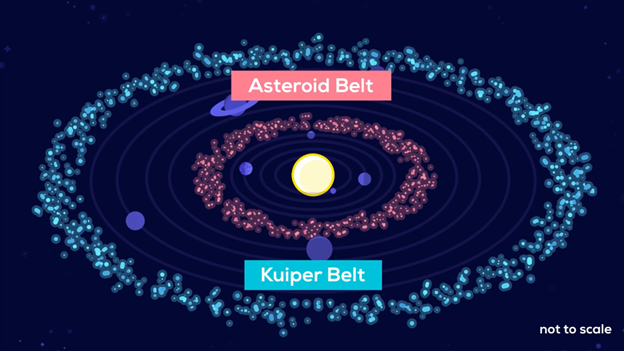
\includegraphics{./images/asteroid-belt.png}
\caption{An illustration of the solar system showing the two asteroid
belts. Image taken from Kurzgesagt}
\end{figure}

Efficiently mining asteroids requires the development of sustainable and
affordable space-grade technology. To achieve this, we must also
identify which asteroids to mine and why. This project focuses on
addressing the latter part of the challenge. Using statistical methods
and techniques, we aim to determine which asteroids can and should be
mined. Our inspiration comes from the insightful Kurzgesagt YouTube
video titled ``Unlimited Resources From Space -- Asteroid Mining.''
{[}1{]}

\hypertarget{dataset}{%
\section{Dataset}\label{dataset}}

To carry out this study we use the data pulled from NASA's Jet
Propulsion Laboratory (JPL), available in Kaggle. ({[}2{]})

\begin{verbatim}
## [1] "Dataset has 839714 rows and 31 columns"
\end{verbatim}

The data set is quite large with nearly 1 million rows of data and 31
different columns.

\hypertarget{column-description}{%
\subsection{Column Description}\label{column-description}}

Let us first introduce the different attributes relevant for our study.
Relevant column names from the dataset are enclosed in paranethesis
after the name of the attribute.

\hypertarget{semi-major-axis-a}{%
\subsubsection{Semi Major Axis (a)}\label{semi-major-axis-a}}

The semi-major axis of an asteroid is the average orbital distance from
the Sun. It is half of the major axis, which is the total distance
between the closest and farthest points of the asteroid's orbit, also
known as the perihelion (q) and aphelion (ad). The semi-major axis is
often measured in astronomical units (AU), with 1 AU defined as the mean
Earth-Sun distance. {[}3{]}

\begin{verbatim}
## [1] "Distribution of values for semi-major axis"
\end{verbatim}

\begin{verbatim}
##       Min.    1st Qu.     Median       Mean    3rd Qu.       Max.       NA's 
## -104279.22       2.39       2.64       2.76       3.00    3043.15          2
\end{verbatim}

\hypertarget{eccentricity-e}{%
\subsubsection{Eccentricity (e)}\label{eccentricity-e}}

The eccentricity of an asteroid is a measure of how much its orbit
deviates from a perfect circle. Orbital shapes can be defined based on
eccentricity value. {[}4{]}

\begin{enumerate}
\def\labelenumi{\arabic{enumi}.}
\item
  Circular orbit: \(e=0\)
\item
  Elliptic orbit: \(0 < e < 1\)
\item
  Parabolic trajectory: \(e = 1\)
\item
  Hyperbolic trajectory: \(e > 1\)
\end{enumerate}

\begin{verbatim}
## [1] "Distribution of values for eccentricity"
\end{verbatim}

\begin{verbatim}
##    Min. 1st Qu.  Median    Mean 3rd Qu.    Max. 
## 0.00000 0.09145 0.14365 0.15564 0.19940 1.20113
\end{verbatim}

\begin{verbatim}
## 
##   Circular Elliptical Hyperbolic  Parabolic 
##          8     839700          4          2
\end{verbatim}

\hypertarget{geometric-albedo-albedo}{%
\subsubsection{Geometric Albedo
(albedo)}\label{geometric-albedo-albedo}}

In astronomy, the geometric albedo of a celestial body is the ratio of
its actual brightness as seen from the light source (i.e., at zero phase
angle) to that of an idealized flat, fully reflecting, diffusively
scattering (Lambertian) disk with the same cross-section. Albedo is
measured on a scale of zero to one, zero representing a surface that
reflects no light, and one representing an object that reflects all
incoming light. {[}5{]}

\begin{verbatim}
## [1] "Distribution of values for eccentricity"
\end{verbatim}

\begin{verbatim}
##    Min. 1st Qu.  Median    Mean 3rd Qu.    Max.    NA's 
##     0.0     0.1     0.1     0.1     0.2     1.0  703305
\end{verbatim}

\hypertarget{absolute-magnitude-parameter-h}{%
\subsubsection{Absolute Magnitude Parameter
(H)}\label{absolute-magnitude-parameter-h}}

Stands for absolute magnitude parameter, denotes the brightness of an
asteroid. It is defined as the apparent magnitude the asteroid would
have if it were observed from the Sun at a distance of 1 Astronomical
Unit (AU). This parameter is used in the calculation of an asteroid's
size. The size of an asteroid can be estimated from its absolute
magnitude (H) and an assumed geometric albedo. {[}6{]}

\begin{verbatim}
## [1] "Distribution of values for absolute magnitude parameter"
\end{verbatim}

\begin{verbatim}
##    Min. 1st Qu.  Median    Mean 3rd Qu.    Max.    NA's 
##   -1.10   15.90   16.80   16.79   17.60   33.20    2689
\end{verbatim}

\hypertarget{magnitude-slope-parameter-g}{%
\subsubsection{Magnitude Slope Parameter
(G)}\label{magnitude-slope-parameter-g}}

The magnitude slope parameter is a component of the \emph{H-G magnitude}
system developed for predicting the magnitude of an asteroid as a
function of solar phase angle. It can also be used for physical studies,
by providing a basis for interpolating or extrapolating brightness from
the phase angles observed at one apparition to the phase angles observed
at another apparition. Thus allowing one to identify the intrinsic
difference in brightness from one apparition to another. This is usually
necessary for studies of asteroid shapes and pole positions. {[}7{]}

\begin{verbatim}
## [1] "Distribution of values for magnitude slope parameter"
\end{verbatim}

\begin{verbatim}
##    Min. 1st Qu.  Median    Mean 3rd Qu.    Max.    NA's 
##    -0.2     0.1     0.2     0.2     0.2     0.6  839595
\end{verbatim}

\hypertarget{color-filters-ub-bv-ir}{%
\subsubsection{Color filters (ub, bv,
ir)}\label{color-filters-ub-bv-ir}}

The three different color index magnitude differences for asteroids.
Each is the difference in magnitude when observed through two filters.

\begin{itemize}
\item
  UB: Ultra-violet and blue filter.
\item
  BV: Blue and Visible (Green) filter.
\item
  IR: Infra-Red filter.
\end{itemize}

\begin{verbatim}
## [1] "Distribution of values for magnitude slope parameter"
\end{verbatim}

\begin{verbatim}
##        UB               BV               IR        
##  Min.   :0.1      Min.   :0.6      Min.   :-0.3    
##  1st Qu.:0.3      1st Qu.:0.7      1st Qu.:-0.3    
##  Median :0.4      Median :0.7      Median :-0.3    
##  Mean   :0.4      Mean   :0.8      Mean   :-0.3    
##  3rd Qu.:0.4      3rd Qu.:0.8      3rd Qu.:-0.3    
##  Max.   :0.7      Max.   :1.1      Max.   :-0.3    
##  NA's   :838735   NA's   :838693   NA's   :839713
\end{verbatim}

These color indices are used to characterize the surface properties of
the asteroid, as different materials reflect light differently at
different wavelengths.

\begin{longtable}[]{@{}
  >{\raggedright\arraybackslash}p{(\columnwidth - 10\tabcolsep) * \real{0.1579}}
  >{\raggedright\arraybackslash}p{(\columnwidth - 10\tabcolsep) * \real{0.1447}}
  >{\raggedright\arraybackslash}p{(\columnwidth - 10\tabcolsep) * \real{0.1842}}
  >{\raggedright\arraybackslash}p{(\columnwidth - 10\tabcolsep) * \real{0.1711}}
  >{\raggedright\arraybackslash}p{(\columnwidth - 10\tabcolsep) * \real{0.1711}}
  >{\raggedright\arraybackslash}p{(\columnwidth - 10\tabcolsep) * \real{0.1711}}@{}}
\toprule\noalign{}
\begin{minipage}[b]{\linewidth}\raggedright
Color Filter
\end{minipage} & \begin{minipage}[b]{\linewidth}\raggedright
C-type
\end{minipage} & \begin{minipage}[b]{\linewidth}\raggedright
M-type
\end{minipage} & \begin{minipage}[b]{\linewidth}\raggedright
S-type
\end{minipage} & \begin{minipage}[b]{\linewidth}\raggedright
Measured Component
\end{minipage} & \begin{minipage}[b]{\linewidth}\raggedright
Higher Value Indicates
\end{minipage} \\
\midrule\noalign{}
\endhead
\bottomrule\noalign{}
\endlastfoot
UB & 0.10 - 0.35 & -0.30 - -0.10 & -0.05 - 0.15 & Iron & More iron
content \\
BV & 0.70 - 1.10 & 0.40 - 0.60 & 0.60 - 0.80 & Pyroxene and Olivine &
More pyroxene and olivine \\
IR & 0.80 - 1.20 & 0.60 - 0.80 & 0.75 - 1.00 & Water Ice & More water
ice \\
\end{longtable}

\hypertarget{orbital-condition-code-condition_code}{%
\subsubsection{Orbital Condition Code
(condition\_code)}\label{orbital-condition-code-condition_code}}

Stands for orbital condition code, also known as the U uncertainty
parameter. Values range from 0 to 9 on the logarithmic scale indicating
how well an object's orbit is known. A value of 0 indicates a
well-determined orbit, while a value of 9 indicates that there are
insufficient observations for long-term orbit prediction. {[}8{]}

\begin{longtable}[]{@{}ll@{}}
\toprule\noalign{}
Condition Code & Orbit Longitude runoff \\
\midrule\noalign{}
\endhead
\bottomrule\noalign{}
\endlastfoot
0 & \textless{} 1.0 arc seconds \\
1 & \textless{} 4.4 arc seconds \\
2 & \textless{} 19.6 arc seconds \\
3 & \textless{} 1.4 arc minutes \\
4 & \textless{} 6.4 arc minutes \\
5 & \textless{} 28.2 arc minutes \\
6 & \textless{} 2.1 degrees \\
7 & \textless{} 9.2 degrees \\
8 & \textless{} 40.7 degrees \\
9 & \textgreater{} 40.7 degrees \\
\end{longtable}

\hypertarget{near-earth-objects-neo}{%
\subsubsection{Near Earth Objects (NEO)}\label{near-earth-objects-neo}}

The value of 1 means the object is near earth, otherwise its 0. There
are 4 types of neos. {[}9{]}

\begin{longtable}[]{@{}lll@{}}
\toprule\noalign{}
Type & Semi-major Axis (AU) & Aphelion Distance (AU) \\
\midrule\noalign{}
\endhead
\bottomrule\noalign{}
\endlastfoot
Atiras & \textless{} 1.1 & \textless{} 1.033 \\
Atens & \textless{} 1.1 & \textgreater{} 1.033 \\
Apollos & \textgreater{} 1.1 & \textless{} 1.307 \\
Amors & \textgreater{} 1.1 & \textgreater{} 1.307 \\
\end{longtable}

\begin{figure}
\centering
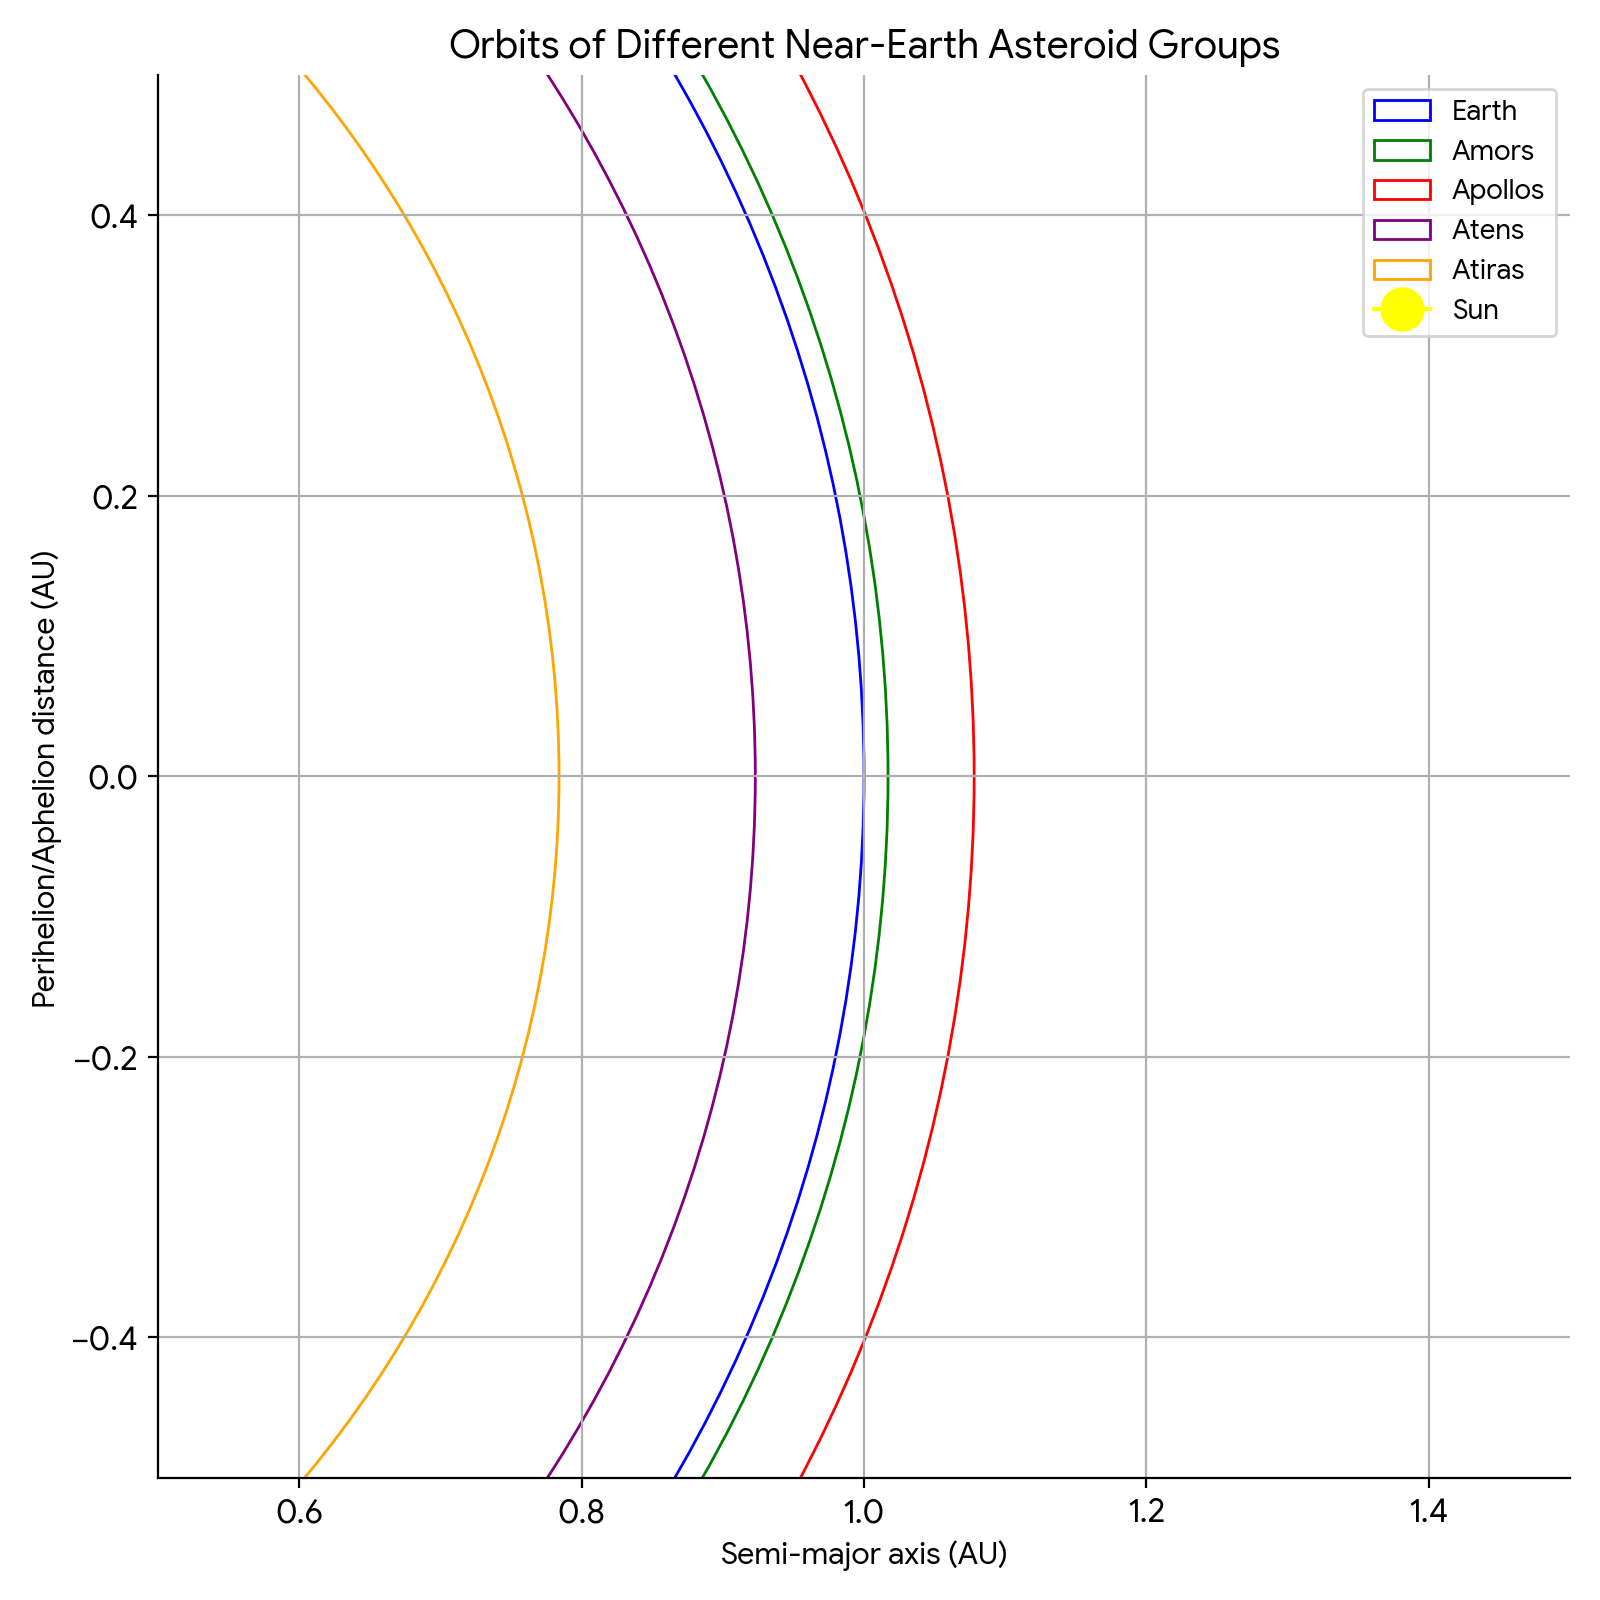
\includegraphics{./images/neo_orbital_paths.png}
\caption{Orbital diagram showing the different types of NEO asteroids}
\end{figure}

\hypertarget{minimum-orbit-intersection-distance-moid}{%
\subsubsection{Minimum Orbit Intersection Distance
(moid)}\label{minimum-orbit-intersection-distance-moid}}

It is a measure used in astronomy to assess potential close approaches
and collision risks between astronomical objects. {[}10{]}

MOID is important to consider for asteroid mining because:

\begin{itemize}
\item
  A lower MOID indicates a closer approach to Earth, potentially
  reducing the cost and travel time for mining missions.
\item
  Consider the frequency and duration of close approaches for efficient
  mission planning.
\item
  Smaller objects may have significantly lower MOIDs, making them more
  accessible.
\end{itemize}

\hypertarget{data-processing}{%
\section{Data Processing}\label{data-processing}}

Before moving forward with our analysis, we first need to process the
dataset.

\hypertarget{attribute-selection}{%
\subsection{Attribute Selection}\label{attribute-selection}}

The dataset contains 31 columns, all of which we don't need. So, we
first select the columns we need and discard the rest.

\begin{Shaded}
\begin{Highlighting}[]
\NormalTok{df }\OtherTok{\textless{}{-}}\NormalTok{ df[}\FunctionTok{c}\NormalTok{(}\StringTok{"a"}\NormalTok{, }\StringTok{"e"}\NormalTok{, }\StringTok{"moid"}\NormalTok{, }\StringTok{"neo"}\NormalTok{, }\StringTok{"condition\_code"}\NormalTok{, }\StringTok{"UB"}\NormalTok{, }\StringTok{"BV"}\NormalTok{, }\StringTok{"IR"}\NormalTok{, }\StringTok{"G"}\NormalTok{, }\StringTok{"H"}\NormalTok{,}
           \StringTok{"albedo"}\NormalTok{, }\StringTok{"diameter"}\NormalTok{, }\StringTok{"per"}\NormalTok{, }\StringTok{"n"}\NormalTok{, }\StringTok{"ad"}\NormalTok{, }\StringTok{"q"}\NormalTok{, }\StringTok{"ma"}\NormalTok{)]}
\FunctionTok{sprintf}\NormalTok{(}\StringTok{"Number of columns in dataset: \%d"}\NormalTok{, }\FunctionTok{ncol}\NormalTok{(df))}
\end{Highlighting}
\end{Shaded}

\begin{verbatim}
## [1] "Number of columns in dataset: 17"
\end{verbatim}

The dataset contains many null values across it's columns. We have to
fill in the missing values as well as we can. Let's first see what
percentage of the columns are missing.

\begin{Shaded}
\begin{Highlighting}[]
\NormalTok{missing\_percentage }\OtherTok{\textless{}{-}} \FunctionTok{colMeans}\NormalTok{(}\FunctionTok{is.na}\NormalTok{(df)) }\SpecialCharTok{*} \DecValTok{100}
\NormalTok{sorted\_missing }\OtherTok{\textless{}{-}} \FunctionTok{sort}\NormalTok{(missing\_percentage, }\AttributeTok{decreasing =} \ConstantTok{TRUE}\NormalTok{)}

\NormalTok{formatted\_missing }\OtherTok{\textless{}{-}} \FunctionTok{sprintf}\NormalTok{(}\StringTok{"\%2.6f\%\%"}\NormalTok{, sorted\_missing)}

\NormalTok{result\_df }\OtherTok{\textless{}{-}} \FunctionTok{data.frame}\NormalTok{(}\AttributeTok{Column =} \FunctionTok{names}\NormalTok{(sorted\_missing), }
                        \AttributeTok{MissingPercentage =}\NormalTok{ formatted\_missing)}
\FunctionTok{print}\NormalTok{(result\_df)}
\end{Highlighting}
\end{Shaded}

\begin{verbatim}
##            Column MissingPercentage
## 1              IR        99.999881%
## 2               G        99.985829%
## 3              UB        99.883413%
## 4              BV        99.878411%
## 5          albedo        83.755302%
## 6        diameter        83.609181%
## 7            moid         1.958048%
## 8               H         0.320228%
## 9              ma         0.000953%
## 10            per         0.000715%
## 11             ad         0.000715%
## 12              a         0.000238%
## 13              n         0.000238%
## 14              e         0.000000%
## 15            neo         0.000000%
## 16 condition_code         0.000000%
## 17              q         0.000000%
\end{verbatim}

Observations:

\begin{itemize}
\item
  albedo, and diameter have over 80\% of missing values. We can use
  regression to fill in these values as best as we can.
\item
  H, e, and a has very few missing values. We can impute with mean.
\item
  condition\_code and neo has no missing values.
\end{itemize}

\hypertarget{discard}{%
\subsection{Discard}\label{discard}}

\hypertarget{columns}{%
\subsubsection{Columns}\label{columns}}

As nearly all the values are missing in G, UB, BV, and IR. We'll be
dropping these columns and won't be using them in our study.

\begin{Shaded}
\begin{Highlighting}[]
\NormalTok{df }\OtherTok{\textless{}{-}}\NormalTok{ df[}\FunctionTok{c}\NormalTok{(}\StringTok{"a"}\NormalTok{, }\StringTok{"e"}\NormalTok{, }\StringTok{"moid"}\NormalTok{, }\StringTok{"neo"}\NormalTok{, }\StringTok{"condition\_code"}\NormalTok{, }\StringTok{"H"}\NormalTok{, }\StringTok{"albedo"}\NormalTok{, }\StringTok{"diameter"}\NormalTok{, }
           \StringTok{"per"}\NormalTok{, }\StringTok{"n"}\NormalTok{, }\StringTok{"ad"}\NormalTok{, }\StringTok{"q"}\NormalTok{, }\StringTok{"ma"}\NormalTok{)]}
\FunctionTok{sprintf}\NormalTok{(}\StringTok{"Number of columns in dataset: \%d"}\NormalTok{, }\FunctionTok{ncol}\NormalTok{(df))}
\end{Highlighting}
\end{Shaded}

\begin{verbatim}
## [1] "Number of columns in dataset: 13"
\end{verbatim}

\hypertarget{rows}{%
\subsubsection{Rows}\label{rows}}

The column condition code has some values that aren't acceptable.
Because we don't know what those values should be, it's easier to just
drop them.

\begin{Shaded}
\begin{Highlighting}[]
\NormalTok{before }\OtherTok{\textless{}{-}} \FunctionTok{nrow}\NormalTok{(df)}
\NormalTok{acceptable\_values }\OtherTok{\textless{}{-}} \FunctionTok{c}\NormalTok{(}\DecValTok{0}\NormalTok{, }\DecValTok{1}\NormalTok{, }\DecValTok{2}\NormalTok{, }\DecValTok{3}\NormalTok{, }\DecValTok{4}\NormalTok{, }\DecValTok{5}\NormalTok{, }\DecValTok{6}\NormalTok{, }\DecValTok{7}\NormalTok{, }\DecValTok{8}\NormalTok{, }\DecValTok{9}\NormalTok{)}
\NormalTok{df }\OtherTok{\textless{}{-}}\NormalTok{ df }\SpecialCharTok{\%\textgreater{}\%} \FunctionTok{filter}\NormalTok{(condition\_code }\SpecialCharTok{\%in\%}\NormalTok{ acceptable\_values)}
\FunctionTok{sprintf}\NormalTok{(}\StringTok{"Dropped \%d rows"}\NormalTok{, before }\SpecialCharTok{{-}} \FunctionTok{nrow}\NormalTok{(df))}
\end{Highlighting}
\end{Shaded}

\begin{verbatim}
## [1] "Dropped 1022 rows"
\end{verbatim}

\hypertarget{imputation}{%
\subsection{Imputation}\label{imputation}}

\hypertarget{impute-numerical-values-using-group-mean}{%
\subsubsection{Impute numerical values using group
mean}\label{impute-numerical-values-using-group-mean}}

The columns H, e, n, ma, and moid have a very small fraction of their
values missing. We'll fill in the missing values based on their
condition code and neo group. This is better than imputing by overall
sample mean.

\begin{Shaded}
\begin{Highlighting}[]
\NormalTok{df }\OtherTok{\textless{}{-}}\NormalTok{ df }\SpecialCharTok{\%\textgreater{}\%} \FunctionTok{group\_by}\NormalTok{(neo, condition\_code) }\SpecialCharTok{\%\textgreater{}\%}
  \FunctionTok{mutate}\NormalTok{(}
    \AttributeTok{H =} \FunctionTok{ifelse}\NormalTok{(}\FunctionTok{is.na}\NormalTok{(H), }\FunctionTok{mean}\NormalTok{(H, }\AttributeTok{na.rm =} \ConstantTok{TRUE}\NormalTok{), H),}
    \AttributeTok{e =} \FunctionTok{ifelse}\NormalTok{(}\FunctionTok{is.na}\NormalTok{(e), }\FunctionTok{mean}\NormalTok{(e, }\AttributeTok{na.rm =} \ConstantTok{TRUE}\NormalTok{), e),}
    \AttributeTok{moid =} \FunctionTok{ifelse}\NormalTok{(}\FunctionTok{is.na}\NormalTok{(moid), }\FunctionTok{mean}\NormalTok{(moid, }\AttributeTok{na.rm =} \ConstantTok{TRUE}\NormalTok{), moid),}
    \AttributeTok{ma =} \FunctionTok{ifelse}\NormalTok{(}\FunctionTok{is.na}\NormalTok{(ma), }\FunctionTok{mean}\NormalTok{(ma, }\AttributeTok{na.rm =} \ConstantTok{TRUE}\NormalTok{), ma),}
    \AttributeTok{ad =} \FunctionTok{ifelse}\NormalTok{(}\FunctionTok{is.na}\NormalTok{(ad), }\FunctionTok{mean}\NormalTok{(ad, }\AttributeTok{na.rm =} \ConstantTok{TRUE}\NormalTok{), ad),}
    \AttributeTok{q =} \FunctionTok{ifelse}\NormalTok{(}\FunctionTok{is.na}\NormalTok{(q), }\FunctionTok{mean}\NormalTok{(q, }\AttributeTok{na.rm =} \ConstantTok{TRUE}\NormalTok{), q)}
\NormalTok{  ) }\SpecialCharTok{\%\textgreater{}\%} \FunctionTok{ungroup}\NormalTok{()}
\end{Highlighting}
\end{Shaded}

\hypertarget{impute-using-regression}{%
\subsubsection{Impute using Regression}\label{impute-using-regression}}

\hypertarget{one-hot-encoding}{%
\paragraph{One hot encoding}\label{one-hot-encoding}}

We first need to convert the categorical columns into separate value
columns using one hot encoding.

\begin{Shaded}
\begin{Highlighting}[]
\NormalTok{df\_encoded }\OtherTok{\textless{}{-}} \FunctionTok{data.frame}\NormalTok{(}\FunctionTok{dummyVars}\NormalTok{(}\StringTok{" \textasciitilde{} ."}\NormalTok{, }\AttributeTok{data =}\NormalTok{ df) }\SpecialCharTok{\%\textgreater{}\%} \FunctionTok{predict}\NormalTok{(df))}
\FunctionTok{sprintf}\NormalTok{(}\StringTok{"Number of columns: \%d"}\NormalTok{, }\FunctionTok{ncol}\NormalTok{(df\_encoded))}
\end{Highlighting}
\end{Shaded}

\begin{verbatim}
## [1] "Number of columns: 23"
\end{verbatim}

\hypertarget{pairwise-column-correlation}{%
\paragraph{Pairwise Column
Correlation}\label{pairwise-column-correlation}}

Now we can calculate pairwise column correlation.

\begin{Shaded}
\begin{Highlighting}[]
\NormalTok{cor\_matrix }\OtherTok{\textless{}{-}} \FunctionTok{cor}\NormalTok{(df\_encoded, }\AttributeTok{use =} \StringTok{"pairwise.complete.obs"}\NormalTok{)}
\FunctionTok{corrplot}\NormalTok{(cor\_matrix, }\AttributeTok{method =} \StringTok{"color"}\NormalTok{)}
\end{Highlighting}
\end{Shaded}

\includegraphics{source_files/figure-latex/Impute_using_regression Finding pairwise correlation between columns-1.png}

Observations:

\begin{enumerate}
\def\labelenumi{\arabic{enumi}.}
\item
  \textbf{neoY} and \textbf{neoN} are entirely negatively correlated,
  which is expected. They come from the same binary column.
\item
  \textbf{H} seems to be somewhat correlated with both \textbf{neo}
  columns.
\item
  \textbf{per} and \textbf{ad} are strongly correlated with \textbf{a}
  and with each other.
\item
  \textbf{q} is strongly correlated with \textbf{moid}.
\end{enumerate}

From these observations, we think that it's better not to use the
\textbf{neo}, \textbf{per}, \textbf{ad}, and \textbf{q} columns when
doing regression.

\hypertarget{creating-regression-models}{%
\paragraph{Creating regression
models}\label{creating-regression-models}}

We'll need two regression models for imputing diameter and albedo.

\begin{Shaded}
\begin{Highlighting}[]
\NormalTok{diameter\_model }\OtherTok{\textless{}{-}} \FunctionTok{lm}\NormalTok{(diameter }\SpecialCharTok{\textasciitilde{}}\NormalTok{ H }\SpecialCharTok{+}\NormalTok{ a }\SpecialCharTok{+}\NormalTok{ e }\SpecialCharTok{+}\NormalTok{ moid }\SpecialCharTok{+}\NormalTok{ condition\_code0 }\SpecialCharTok{+} 
\NormalTok{                       condition\_code2 }\SpecialCharTok{+}\NormalTok{  condition\_code6 }\SpecialCharTok{+}\NormalTok{ condition\_code7 }\SpecialCharTok{+} 
\NormalTok{                       condition\_code8,}
                     \AttributeTok{data =}\NormalTok{ df\_encoded[}\SpecialCharTok{!}\FunctionTok{is.na}\NormalTok{(df\_encoded}\SpecialCharTok{$}\NormalTok{diameter), ])}

\FunctionTok{summary}\NormalTok{(diameter\_model)}
\end{Highlighting}
\end{Shaded}

\begin{verbatim}
## 
## Call:
## lm(formula = diameter ~ H + a + e + moid + condition_code0 + 
##     condition_code2 + condition_code6 + condition_code7 + condition_code8, 
##     data = df_encoded[!is.na(df_encoded$diameter), ])
## 
## Residuals:
##    Min     1Q Median     3Q    Max 
## -39.98  -2.47  -0.49   1.60 891.02 
## 
## Coefficients:
##                 Estimate Std. Error  t value Pr(>|t|)    
## (Intercept)     56.91236    0.31446  180.986  < 2e-16 ***
## H               -3.69810    0.01615 -228.935  < 2e-16 ***
## a               -0.08312    0.01466   -5.668 1.44e-08 ***
## e               19.24813    0.30844   62.404  < 2e-16 ***
## moid             3.96701    0.05254   75.501  < 2e-16 ***
## condition_code0 -3.73994    0.08704  -42.970  < 2e-16 ***
## condition_code2  1.93703    0.38497    5.032 4.87e-07 ***
## condition_code6  1.51148    0.54940    2.751  0.00594 ** 
## condition_code7  1.61709    0.52433    3.084  0.00204 ** 
## condition_code8  5.50128    0.85354    6.445 1.16e-10 ***
## ---
## Signif. codes:  0 '***' 0.001 '**' 0.01 '*' 0.05 '.' 0.1 ' ' 1
## 
## Residual standard error: 7.447 on 137626 degrees of freedom
## Multiple R-squared:  0.3704, Adjusted R-squared:  0.3704 
## F-statistic:  8997 on 9 and 137626 DF,  p-value: < 2.2e-16
\end{verbatim}

Here, we have kept only the parameters that are statistically
significant at \(\alpha=0.01\). The rest have been removed from the
linear regression model.

In the same way, we'll create a model for albedo as well.

\begin{Shaded}
\begin{Highlighting}[]
\NormalTok{albedo\_model }\OtherTok{\textless{}{-}} \FunctionTok{lm}\NormalTok{(albedo }\SpecialCharTok{\textasciitilde{}}\NormalTok{ H }\SpecialCharTok{+}\NormalTok{ a }\SpecialCharTok{+}\NormalTok{ e }\SpecialCharTok{+}\NormalTok{ moid }\SpecialCharTok{+}\NormalTok{ condition\_code0 }\SpecialCharTok{+} 
\NormalTok{                     condition\_code1 }\SpecialCharTok{+}\NormalTok{  condition\_code2 }\SpecialCharTok{+}\NormalTok{ condition\_code3 }\SpecialCharTok{+} 
\NormalTok{                     condition\_code4 }\SpecialCharTok{+}\NormalTok{  condition\_code5 }\SpecialCharTok{+}\NormalTok{ condition\_code6 }\SpecialCharTok{+} 
\NormalTok{                     condition\_code7 }\SpecialCharTok{+}\NormalTok{  condition\_code8,}
                     \AttributeTok{data =}\NormalTok{ df\_encoded[}\SpecialCharTok{!}\FunctionTok{is.na}\NormalTok{(df\_encoded}\SpecialCharTok{$}\NormalTok{albedo), ])}

\FunctionTok{summary}\NormalTok{(albedo\_model)}
\end{Highlighting}
\end{Shaded}

\begin{verbatim}
## 
## Call:
## lm(formula = albedo ~ H + a + e + moid + condition_code0 + condition_code1 + 
##     condition_code2 + condition_code3 + condition_code4 + condition_code5 + 
##     condition_code6 + condition_code7 + condition_code8, data = df_encoded[!is.na(df_encoded$albedo), 
##     ])
## 
## Residuals:
##     Min      1Q  Median      3Q     Max 
## -0.5272 -0.0603 -0.0268  0.0448  3.7639 
## 
## Coefficients:
##                   Estimate Std. Error  t value Pr(>|t|)    
## (Intercept)      0.7441832  0.0040833  182.249  < 2e-16 ***
## H               -0.0298707  0.0002088 -143.047  < 2e-16 ***
## a                0.0025335  0.0001887   13.423  < 2e-16 ***
## e               -0.3000713  0.0040414  -74.250  < 2e-16 ***
## moid            -0.1142782  0.0006813 -167.743  < 2e-16 ***
## condition_code0  0.0393011  0.0013037   30.147  < 2e-16 ***
## condition_code1  0.0463547  0.0029514   15.706  < 2e-16 ***
## condition_code2  0.0921228  0.0050747   18.153  < 2e-16 ***
## condition_code3  0.1060818  0.0077557   13.678  < 2e-16 ***
## condition_code4  0.0550493  0.0074903    7.349 2.00e-13 ***
## condition_code5  0.0418575  0.0054805    7.638 2.23e-14 ***
## condition_code6  0.0418266  0.0072916    5.736 9.70e-09 ***
## condition_code7  0.0608222  0.0068614    8.864  < 2e-16 ***
## condition_code8  0.1151087  0.0110723   10.396  < 2e-16 ***
## ---
## Signif. codes:  0 '***' 0.001 '**' 0.01 '*' 0.05 '.' 0.1 ' ' 1
## 
## Residual standard error: 0.09578 on 136395 degrees of freedom
## Multiple R-squared:  0.2419, Adjusted R-squared:  0.2418 
## F-statistic:  3347 on 13 and 136395 DF,  p-value: < 2.2e-16
\end{verbatim}

Both of our models have a p-value of less than \(2^{-16}\). Which means,
they are very good at predicting the values of diameter and albedo
respectively. Now we use them to fill in the missing values

\begin{Shaded}
\begin{Highlighting}[]
\NormalTok{missing\_values }\OtherTok{\textless{}{-}} \FunctionTok{is.na}\NormalTok{(df}\SpecialCharTok{$}\NormalTok{diameter)}
\NormalTok{impute\_data }\OtherTok{\textless{}{-}}\NormalTok{ df\_encoded[missing\_values, ]}
\NormalTok{imputed\_values }\OtherTok{\textless{}{-}} \FunctionTok{predict}\NormalTok{(diameter\_model, }\AttributeTok{newdata =}\NormalTok{ impute\_data)}
\NormalTok{df}\SpecialCharTok{$}\NormalTok{diameter[missing\_values] }\OtherTok{\textless{}{-}}\NormalTok{ imputed\_values}

\NormalTok{missing\_values }\OtherTok{\textless{}{-}} \FunctionTok{is.na}\NormalTok{(df}\SpecialCharTok{$}\NormalTok{albedo)}
\NormalTok{impute\_data }\OtherTok{\textless{}{-}}\NormalTok{ df\_encoded[missing\_values, ]}
\NormalTok{imputed\_values }\OtherTok{\textless{}{-}} \FunctionTok{predict}\NormalTok{(albedo\_model, }\AttributeTok{newdata =}\NormalTok{ impute\_data)}
\NormalTok{df}\SpecialCharTok{$}\NormalTok{albedo[missing\_values] }\OtherTok{\textless{}{-}}\NormalTok{ imputed\_values}
\end{Highlighting}
\end{Shaded}

\hypertarget{custom-columns}{%
\subsection{Custom Columns}\label{custom-columns}}

\hypertarget{distance-from-earth}{%
\subsubsection{Distance From Earth}\label{distance-from-earth}}

The distance from earth (d) can be calculated using semi-major axis (a)
and eccentricity (e). The formula is as follows

\[
d = a \times (1 - e)
\]

\begin{Shaded}
\begin{Highlighting}[]
\NormalTok{df}\SpecialCharTok{$}\NormalTok{d }\OtherTok{\textless{}{-}}\NormalTok{ df}\SpecialCharTok{$}\NormalTok{a }\SpecialCharTok{*}\NormalTok{ (}\DecValTok{1} \SpecialCharTok{{-}}\NormalTok{ df}\SpecialCharTok{$}\NormalTok{e)}
\FunctionTok{summary}\NormalTok{(df}\SpecialCharTok{$}\NormalTok{d)}
\end{Highlighting}
\end{Shaded}

\begin{verbatim}
##     Min.  1st Qu.   Median     Mean  3rd Qu.     Max. 
##  0.07051  1.97218  2.22574  2.40488  2.57836 80.42417
\end{verbatim}

\hypertarget{material-group}{%
\subsubsection{Material Group}\label{material-group}}

Based on geometric albedo, we can approximately guess what type an
asteroid is.

\begin{longtable}[]{@{}
  >{\raggedright\arraybackslash}p{(\columnwidth - 4\tabcolsep) * \real{0.1806}}
  >{\raggedright\arraybackslash}p{(\columnwidth - 4\tabcolsep) * \real{0.1667}}
  >{\raggedright\arraybackslash}p{(\columnwidth - 4\tabcolsep) * \real{0.6528}}@{}}
\toprule\noalign{}
\begin{minipage}[b]{\linewidth}\raggedright
Asteroid Type
\end{minipage} & \begin{minipage}[b]{\linewidth}\raggedright
Albedo Range
\end{minipage} & \begin{minipage}[b]{\linewidth}\raggedright
Major Components
\end{minipage} \\
\midrule\noalign{}
\endhead
\bottomrule\noalign{}
\endlastfoot
C-type & 0.03 - 0.10 & Carbon, silicates, water ice, organic
compounds \\
M-type & 0.10 - 0.30 & Nickel-iron, iron sulfide \\
S-type & 0.10 - 0.25 & Silicates, iron-nickel \\
\end{longtable}

Based on this, we can say that asteroids are mostly of two material
types: Carbonaceous or Metalic. C-type is carbonaceous while others are
metallic.

\begin{verbatim}
## 
## carbonaceous     metallic 
##       485398       353294
\end{verbatim}

\hypertarget{neo-type}{%
\subsubsection{NEO Type}\label{neo-type}}

In this section, we create a column to represent the 4 NEO types.

\begin{Shaded}
\begin{Highlighting}[]
\NormalTok{define\_neo\_type }\OtherTok{\textless{}{-}} \ControlFlowTok{function}\NormalTok{(a, ad) \{}
  \FunctionTok{ifelse}\NormalTok{(a }\SpecialCharTok{\textless{}} \FloatTok{1.1}\NormalTok{,}
         \FunctionTok{ifelse}\NormalTok{(ad }\SpecialCharTok{\textless{}} \FloatTok{1.033}\NormalTok{, }\StringTok{"Atiras"}\NormalTok{, }\StringTok{"Atens"}\NormalTok{),}
         \FunctionTok{ifelse}\NormalTok{(ad }\SpecialCharTok{\textless{}} \FloatTok{1.307}\NormalTok{, }\StringTok{"Apollos"}\NormalTok{, }\StringTok{"Amors"}\NormalTok{))}
\NormalTok{\}}

\NormalTok{df }\OtherTok{\textless{}{-}}\NormalTok{ df }\SpecialCharTok{\%\textgreater{}\%} \FunctionTok{rowwise}\NormalTok{() }\SpecialCharTok{\%\textgreater{}\%} \FunctionTok{mutate}\NormalTok{(}\AttributeTok{neo\_type =} \FunctionTok{define\_neo\_type}\NormalTok{(a, ad))}
\FunctionTok{table}\NormalTok{(df}\SpecialCharTok{$}\NormalTok{neo\_type)}
\end{Highlighting}
\end{Shaded}

\begin{verbatim}
## 
##   Amors Apollos   Atens  Atiras 
##  835778     259    2469     186
\end{verbatim}

\hypertarget{exploratory-data-analysis}{%
\section{Exploratory Data Analysis}\label{exploratory-data-analysis}}

In this section we'd like to go over the different factors that play
into asteroid mining. In particular, we try to answer the following
question from a feasibility stand point:

\begin{enumerate}
\def\labelenumi{\arabic{enumi}.}
\item
  \textbf{Distance}: It's easier to mine asteroids the closer they are.
  On average, is the mean distance of NEO asteroids less than 1 AU?
\item
  \textbf{Material}: Metallic resources are more valuable and thus
  metallic asteroids should be sought out for mining. Does NEO asteroids
  have proportionately more metallic asteroids than non-NEO asteroids?
\item
  \textbf{Asteroid size}: Large asteroids have more resources than
  smaller asteroids. On average, is the mean diameter of NEO asteroids
  smaller than non-NEO asteroids?
\item
  \textbf{Diameter difference}: There are 4 different types of NEO
  asteroids. Is there a significant difference between their average
  diameter?
\item
  \textbf{Value difference}: From a material value standpoint, which NEO
  type is the best to mine?
\end{enumerate}

\hypertarget{distance-from-earth-1}{%
\subsection{Distance from Earth}\label{distance-from-earth-1}}

Asteroid mining is feasible for asteroid which are close to earth. This
means we want to consider only NEO or Near Earth Object asteroids for
our initial mining operations. The closer an asteroid is to earth the
cheaper it is for us due to lower cost in transportation. A good
starting point would be to mine asteroids that are at most 1 AU from
earth. This is the same distance from the earth to the sun. We want to
know if all NEO asteroids are on average at most 1 AU away from earth.
Meaning, our hypothesis is as follows: (Here, \(\mu_d\) represents the
average distance for NEO asteroids)

\begin{itemize}
\item
  Null hypothesis: \(\mathbf{H_0}: \mu_d \ge 1.0\). In other words, NEO
  asteroids are on average more than 1 AU distance from earth.
\item
  Alternative hypothesis: \(\mathbf{H_1}: \mu_d < 1.0\). In other words,
  NEO asteroids are on average less than 1 AU distance from earth.
\end{itemize}

As we have a large dataset, we want to be very conservative. We want to
be 99.99\% confident. Which means our significance level is
\(\alpha = 0.0001\).

Let's take a look at the distribution of distances of NEO asteroids:

\begin{Shaded}
\begin{Highlighting}[]
\NormalTok{plot\_distance\_hist }\OtherTok{\textless{}{-}} \ControlFlowTok{function}\NormalTok{(df, xlabel) \{}
\NormalTok{  mean\_d }\OtherTok{\textless{}{-}} \FunctionTok{mean}\NormalTok{(df}\SpecialCharTok{$}\NormalTok{d)}
\NormalTok{  median\_d }\OtherTok{\textless{}{-}} \FunctionTok{median}\NormalTok{(df}\SpecialCharTok{$}\NormalTok{d)}
  
  \FunctionTok{ggplot}\NormalTok{(df, }\FunctionTok{aes}\NormalTok{(}\AttributeTok{x=}\NormalTok{d)) }\SpecialCharTok{+}
    \FunctionTok{geom\_histogram}\NormalTok{(}\AttributeTok{bins =} \FunctionTok{ceiling}\NormalTok{(}\FunctionTok{log}\NormalTok{(}\FunctionTok{length}\NormalTok{(df}\SpecialCharTok{$}\NormalTok{d))) }\SpecialCharTok{+} \DecValTok{1}\NormalTok{) }\SpecialCharTok{+}
    \FunctionTok{geom\_vline}\NormalTok{(}\FunctionTok{aes}\NormalTok{(}\AttributeTok{xintercept =}\NormalTok{ mean\_d, }\AttributeTok{color =} \StringTok{"red"}\NormalTok{), }\AttributeTok{show.legend =}\NormalTok{ F) }\SpecialCharTok{+}
    \FunctionTok{annotate}\NormalTok{(}\StringTok{"text"}\NormalTok{, }\AttributeTok{x=}\NormalTok{mean\_d}\FloatTok{+0.1}\NormalTok{, }\AttributeTok{y=}\DecValTok{3500}\NormalTok{, }
             \AttributeTok{label=}\FunctionTok{substitute}\NormalTok{(}\FunctionTok{paste}\NormalTok{(}\FunctionTok{bar}\NormalTok{(x),}\StringTok{"="}\NormalTok{,m), }
                              \FunctionTok{list}\NormalTok{(}\AttributeTok{m=}\FunctionTok{sprintf}\NormalTok{(}\StringTok{"\%.02f"}\NormalTok{, mean\_d))), }
             \AttributeTok{col=}\StringTok{"red"}\NormalTok{) }\SpecialCharTok{+}
    \FunctionTok{geom\_vline}\NormalTok{(}\FunctionTok{aes}\NormalTok{(}\AttributeTok{xintercept =}\NormalTok{ median\_d, }\AttributeTok{color =} \StringTok{"blue"}\NormalTok{), }\AttributeTok{show.legend =}\NormalTok{ F) }\SpecialCharTok{+}
    \FunctionTok{annotate}\NormalTok{(}\StringTok{"text"}\NormalTok{, }\AttributeTok{x=}\NormalTok{median\_d}\FloatTok{{-}0.1}\NormalTok{, }\AttributeTok{y=}\DecValTok{3500}\NormalTok{, }
             \AttributeTok{label=}\FunctionTok{substitute}\NormalTok{(}\FunctionTok{paste}\NormalTok{(}\FunctionTok{tilde}\NormalTok{(x),}\StringTok{"="}\NormalTok{,m), }
                              \FunctionTok{list}\NormalTok{(}\AttributeTok{m=}\FunctionTok{sprintf}\NormalTok{(}\StringTok{"\%.02f"}\NormalTok{, median\_d))), }
             \AttributeTok{col=}\StringTok{"blue"}\NormalTok{) }\SpecialCharTok{+}
    \FunctionTok{labs}\NormalTok{(}\AttributeTok{title =} \StringTok{"Histogram of Distance from Earth"}\NormalTok{,}
         \AttributeTok{subtitle =} \StringTok{"For Near Earth Object (NEO) asteroids"}\NormalTok{) }\SpecialCharTok{+}
    \FunctionTok{xlab}\NormalTok{(xlabel) }\SpecialCharTok{+}
    \FunctionTok{ylab}\NormalTok{(}\StringTok{"Count"}\NormalTok{) }\SpecialCharTok{+}
    \FunctionTok{theme}\NormalTok{(}\AttributeTok{plot.title =} \FunctionTok{element\_text}\NormalTok{(}\AttributeTok{hjust =} \FloatTok{0.5}\NormalTok{),}
          \AttributeTok{plot.subtitle =} \FunctionTok{element\_text}\NormalTok{(}\AttributeTok{hjust =} \FloatTok{0.5}\NormalTok{))}
\NormalTok{\}}

\NormalTok{df\_temp }\OtherTok{\textless{}{-}}\NormalTok{ df[df}\SpecialCharTok{$}\NormalTok{neo }\SpecialCharTok{==} \StringTok{\textquotesingle{}Y\textquotesingle{}}\NormalTok{, }\StringTok{\textquotesingle{}d\textquotesingle{}}\NormalTok{]}
\FunctionTok{plot\_distance\_hist}\NormalTok{(df\_temp, }\StringTok{"Distance from Earth (AU)"}\NormalTok{)}
\end{Highlighting}
\end{Shaded}

\begin{verbatim}
## Warning in is.na(x): is.na() applied to non-(list or vector) of type 'language'

## Warning in is.na(x): is.na() applied to non-(list or vector) of type 'language'
\end{verbatim}

\includegraphics{source_files/figure-latex/EDA distance from earth histogram-1.png}

The distribution of the distance appears to be left skewed. We'll make
it more symmetrical shape using boxcox transformation.

\begin{Shaded}
\begin{Highlighting}[]
\NormalTok{bcl\_d }\OtherTok{=} \FunctionTok{boxcox}\NormalTok{(df\_temp}\SpecialCharTok{$}\NormalTok{d}\SpecialCharTok{\textasciitilde{}}\DecValTok{1}\NormalTok{)}
\end{Highlighting}
\end{Shaded}

\includegraphics{source_files/figure-latex/EDA boxcox to make distance normal shaped-1.png}

\begin{Shaded}
\begin{Highlighting}[]
\NormalTok{lambda\_d }\OtherTok{=}\NormalTok{ bcl\_d}\SpecialCharTok{$}\NormalTok{x[bcl\_d}\SpecialCharTok{$}\NormalTok{y }\SpecialCharTok{==} \FunctionTok{max}\NormalTok{(bcl\_d}\SpecialCharTok{$}\NormalTok{y)]}
\NormalTok{df\_temp}\SpecialCharTok{$}\NormalTok{d }\OtherTok{=}\NormalTok{ (df\_temp}\SpecialCharTok{$}\NormalTok{d }\SpecialCharTok{\^{}}\NormalTok{ lambda\_d }\SpecialCharTok{{-}} \DecValTok{1}\NormalTok{) }\SpecialCharTok{/}\NormalTok{ lambda\_d}
\end{Highlighting}
\end{Shaded}

Now the distribution should look much more normally distributed.

\begin{verbatim}
## Warning in is.na(x): is.na() applied to non-(list or vector) of type 'language'

## Warning in is.na(x): is.na() applied to non-(list or vector) of type 'language'
\end{verbatim}

\includegraphics{source_files/figure-latex/EDA distance from earth histogram after boxcox-1.png}

Now that our data is normal, we can move forward with the hypothesis
test. We'll be doing a one sample t-test. As we don't know the
population variance, we can't do a z-test.

\begin{Shaded}
\begin{Highlighting}[]
\FunctionTok{t.test}\NormalTok{(}\AttributeTok{x =}\NormalTok{ df\_temp}\SpecialCharTok{$}\NormalTok{d, }\AttributeTok{alternative =} \StringTok{"less"}\NormalTok{, }\AttributeTok{conf.level =} \DecValTok{1}\FloatTok{{-}0.0001}\NormalTok{, }
       \AttributeTok{mu =}\NormalTok{ (}\DecValTok{1} \SpecialCharTok{\^{}}\NormalTok{ lambda\_d }\SpecialCharTok{{-}} \DecValTok{1}\NormalTok{) }\SpecialCharTok{/}\NormalTok{ lambda\_d)}
\end{Highlighting}
\end{Shaded}

\begin{verbatim}
## 
##  One Sample t-test
## 
## data:  df_temp$d
## t = -41.106, df = 21398, p-value < 2.2e-16
## alternative hypothesis: true mean is less than 0
## 99.99 percent confidence interval:
##         -Inf -0.05067877
## sample estimates:
##  mean of x 
## -0.0557209
\end{verbatim}

The p-value is \(2.2^{-16}\) which is much smaller than our level of
significance. Thus, we have significant evidence to reject the null
hypothesis.

\begin{Shaded}
\begin{Highlighting}[]
\NormalTok{upper\_bound }\OtherTok{\textless{}{-}}\NormalTok{ (}\SpecialCharTok{{-}}\FloatTok{0.05067877} \SpecialCharTok{*}\NormalTok{ lambda\_d }\SpecialCharTok{+} \DecValTok{1}\NormalTok{) }\SpecialCharTok{\^{}}\NormalTok{ (}\DecValTok{1} \SpecialCharTok{/}\NormalTok{ lambda\_d)}
\FunctionTok{sprintf}\NormalTok{(}\StringTok{"Confidence Interval in original scale: ({-}inf, \%.4f)"}\NormalTok{, upper\_bound)}
\end{Highlighting}
\end{Shaded}

\begin{verbatim}
## [1] "Confidence Interval in original scale: (-inf, 0.9481)"
\end{verbatim}

Meaning, NEO asteroids on average are at most 0.9481 AU from earth.

\hypertarget{verdict}{%
\subsubsection{Verdict}\label{verdict}}

Most near earth asteroids are at most 1 AU from our planet. That's great
news for asteroids mining as we don't have to spend a lot on space
travel to find asteroids to mine.

\hypertarget{material-value}{%
\subsection{Material Value}\label{material-value}}

Metals, like iron, nickel, gold, platinum, are the building block of our
civilization. They are precious resources and will be highly valuable to
mine from asteroids. Asteroids composed of metals are thus highly
valuable. So for asteroid mining to be feasible we might want to seek
out and mine metallic asteroids more than carbonaceous ones. However,
most asteroids we know are carbonaceous. In accordance with out previous
decision then, it doesn't make much sense to go mine asteroids that
aren't NEO as most of those will be carbonaceous while being far away.
We'd like to test this claim with a two-sample proportion test.

\begin{itemize}
\item
  Null Hypothesis: \(\mathbf{H_0}: p_c \le p_f\) which means the
  proportion of metallic NEO asteroids (\(p_c\)) are less than or equal
  to the proportion of metallic non-NEO asteroids (\(p_f\)).
\item
  Alternative Hypothesis: \(\mathbf{H_1}: p_c > p_f\) which means the
  proportion of metallic NEO asteroids (\(p_c\)) are greater the
  proportion of metallic non-NEO asteroids (\(p_f\)).
\end{itemize}

As before, because we have a lot of samples, we want to be very
confident, about 99.99\%. Meaning, our significance level is
\(\alpha = 0.0001\).

We begin by visually looking at the distribution of different types of
asteroids.

\includegraphics{source_files/figure-latex/EDA Bar chart for material distribution-1.png}

From the bar chart, it looks like that a higher proportion of non-NEO
asteroids are metallic, which aligns with the null hypothesis. Let's see
if we can statistically reject it.

\begin{verbatim}
## 
##  2-sample test for equality of proportions without continuity correction
## 
## data:  c(x_c, x_f) out of c(n_c, n_f)
## X-squared = 10209, df = 1, p-value = 1
## alternative hypothesis: greater
## 99.99 percent confidence interval:
##  -0.352837  1.000000
## sample estimates:
##     prop 1     prop 2 
## 0.08458339 0.43005874
\end{verbatim}

Since the p-value is greater than our confidence level, we fail to
reject the null hypothesis. Meaning, a greater proportion of non-NEO
asteroids are metallic than NEO asteroids.

\hypertarget{verdict-1}{%
\subsubsection{Verdict}\label{verdict-1}}

This test allows us to see the trade off between distance and value. It
proves that we are more likely to get highly valuable asteroids when we
don't limit ourselves to near earth asteroids. This is because a greater
proportion of asteroids that are not NEO are metallic and these are
highly desirable asteroids.

\hypertarget{asteroid-size}{%
\subsection{Asteroid size}\label{asteroid-size}}

An important consideration when mining asteroids is the size of the
asteroid. Typically, a large asteroid will have more valuable materials
than a smaller asteroid. It is thus important to know where the larger
asteroids lie, near or far away from earth. We want to test if the
asteroids near earth are smaller than the asteroids far away from earth.
So our hypothesis are

\begin{itemize}
\item
  Null Hypothesis: TODO
\item
  Alternative Hypothesis: TODO
\end{itemize}

We're going to carry out this hypothesis test using a two-sample t-test
or Welch Test with \(\alpha = 0.0001\).

\begin{Shaded}
\begin{Highlighting}[]
\CommentTok{\# }\AlertTok{TODO}\CommentTok{: Visualization}
\end{Highlighting}
\end{Shaded}

\begin{Shaded}
\begin{Highlighting}[]
\CommentTok{\# }\AlertTok{TODO}\CommentTok{: Transformation (if required)}
\end{Highlighting}
\end{Shaded}

\begin{Shaded}
\begin{Highlighting}[]
\CommentTok{\# }\AlertTok{TODO}\CommentTok{: Hypothesis testing (Two{-}sample t{-}test)}
\end{Highlighting}
\end{Shaded}

\hypertarget{verdict-2}{%
\subsubsection{Verdict}\label{verdict-2}}

\hypertarget{diameter-difference}{%
\subsection{Diameter Difference}\label{diameter-difference}}

There are 4 different types of NEOs based on semi-major axis and
aphelion distance: Amors, Apollos, Atens, and Atiras. Amos is the
closest to earth's orbit while Atiras is the furthest away. We want to
see if the size of the asteroids vary across these 4 types. Meaning,
we'd like to do a hypothesis test using ANOVA, where we check if the
average diameter of asteroids is different among these 4 types of
asteroids. If so, we'd like to know which NEO asteroids are on average
larger from pairwise t-tests. Thus our hypothesis is as follows:

\begin{itemize}
\item
  Null Hypothesis: \$\mathbf{H_0}: \mu\_1 = \mu\_2 = \mu\_3 = \mu\_4 \$.
  There is no significant difference in the average diameter of
  asteroids among the four types (Amors, Apollos, Atens, and Atiras).
\item
  Alternative Hypothesis: \$\mathbf{H_1}: \text{At least one } \mu\_i
  \text{ is different} \$ There is a significant difference in the
  average diameter of asteroids among the four types (Amors, Apollos,
  Atens, and Atiras).
\end{itemize}

We're going to carry out this hypothesis test with \(\alpha = 0.0001\).

\begin{Shaded}
\begin{Highlighting}[]
\CommentTok{\# }\AlertTok{TODO}\CommentTok{: Visualization}
\end{Highlighting}
\end{Shaded}

\begin{Shaded}
\begin{Highlighting}[]
\CommentTok{\# }\AlertTok{TODO}\CommentTok{: Transformation (if required)}
\end{Highlighting}
\end{Shaded}

\begin{Shaded}
\begin{Highlighting}[]
\CommentTok{\# }\AlertTok{TODO}\CommentTok{: Hypothesis testing (One{-}way ANOVA)}
\end{Highlighting}
\end{Shaded}

\hypertarget{verdict-3}{%
\subsubsection{Verdict}\label{verdict-3}}

\hypertarget{value-difference}{%
\subsection{Value Difference}\label{value-difference}}

Among the 4 different types of NEO asteroids, we want to determine which
type has most percentage of metallic asteroids. The more metallic
asteroid, the better our chance of mining precious materials. For this,
we're going to a chisqaure test of independence. We want to find
distinctions in proportions among the different asteroid types and then
find which one has the highest. Our hypothesis is as follows:

\begin{itemize}
\item
  Null Hypothesis: TODO
\item
  Alternative Hypothesis: TODO
\end{itemize}

We're going to carry out this hypothesis test with \(\alpha = 0.0001\).

\begin{Shaded}
\begin{Highlighting}[]
\CommentTok{\# }\AlertTok{TODO}\CommentTok{: Visualization}
\end{Highlighting}
\end{Shaded}

\begin{Shaded}
\begin{Highlighting}[]
\CommentTok{\# }\AlertTok{TODO}\CommentTok{: Transformation (if required)}
\end{Highlighting}
\end{Shaded}

\begin{Shaded}
\begin{Highlighting}[]
\CommentTok{\# }\AlertTok{TODO}\CommentTok{: Hypothesis testing (chisqaure test of independence)}
\end{Highlighting}
\end{Shaded}

\hypertarget{verdict-4}{%
\subsubsection{Verdict}\label{verdict-4}}

\hypertarget{conclusion}{%
\section{Conclusion}\label{conclusion}}

\hypertarget{references}{%
\section*{References}\label{references}}
\addcontentsline{toc}{section}{References}

\hypertarget{refs}{}
\begin{CSLReferences}{0}{0}
\leavevmode\vadjust pre{\hypertarget{ref-Kurzgesagt2020}{}}%
\CSLLeftMargin{{[}1{]} }%
\CSLRightInline{K. --In a Nutshell, {``Unlimited resources from space --
asteroid mining.''} YouTube, 2020. Available:
\url{http://www.youtube.com/watch?v=y8XvQNt26KI}}

\leavevmode\vadjust pre{\hypertarget{ref-OpenAsteroidDataBasu2019}{}}%
\CSLLeftMargin{{[}2{]} }%
\CSLRightInline{V. BASU, {``Open asteroid dataset.''} Kaggle, 2019.
Available:
\url{https://www.kaggle.com/datasets/basu369victor/prediction-of-asteroid-diameter}}

\leavevmode\vadjust pre{\hypertarget{ref-NASAOrbitsKeplersLaws2023}{}}%
\CSLLeftMargin{{[}3{]} }%
\CSLRightInline{{``Orbits and kepler's laws.''} National Aeronautics;
Space Administration (NASA), 2023. Available:
\url{https://science.nasa.gov/resource/orbits-and-keplers-laws/}}

\leavevmode\vadjust pre{\hypertarget{ref-WikipediaOrbitalEccentricity2023}{}}%
\CSLLeftMargin{{[}4{]} }%
\CSLRightInline{{``Orbital eccentricity.''} Wikipedia, 2023. Available:
\url{https://en.wikipedia.org/wiki/Orbital_eccentricity}}

\leavevmode\vadjust pre{\hypertarget{ref-WikipediaGeometricAlbedo2023}{}}%
\CSLLeftMargin{{[}5{]} }%
\CSLRightInline{{``Geometric albedo.''} Wikipedia, 2023. Available:
\url{https://en.wikipedia.org/wiki/Geometric_albedo}}

\leavevmode\vadjust pre{\hypertarget{ref-NASACNEOSAsteroidSizeEstimator2023}{}}%
\CSLLeftMargin{{[}6{]} }%
\CSLRightInline{{``Asteroid size estimator.''} National Aeronautics;
Space Administration (NASA) Center for Near-Earth Object Studies
(CNEOS), 2023. Available:
\url{https://cneos.jpl.nasa.gov/tools/ast_size_est.html}}

\leavevmode\vadjust pre{\hypertarget{ref-Harris1989}{}}%
\CSLLeftMargin{{[}7{]} }%
\CSLRightInline{A. W. Harris, {``THE h-g ASTEROID MAGNITUDE SYSTEM: MEAN
SLOPE PARAMETERS,''} \emph{Lunar and Planetary Science Conference}, vol.
20, pp. 407--408, 1989, doi:
\href{https://doi.org/10.21236/lunaplanet.19890076}{10.21236/lunaplanet.19890076}.}

\leavevmode\vadjust pre{\hypertarget{ref-NASATrajectoryBrowserUserGuide2023}{}}%
\CSLLeftMargin{{[}8{]} }%
\CSLRightInline{{``Trajectory browser user guide.''} National
Aeronautics; Space Administration (NASA) Ames Research Center, 2023.
Available: \url{https://trajbrowser.arc.nasa.gov/user_guide.php}}

\leavevmode\vadjust pre{\hypertarget{ref-NASACNEOSNEOGroups2023}{}}%
\CSLLeftMargin{{[}9{]} }%
\CSLRightInline{{``Near-earth object (NEO) groups.''} National
Aeronautics; Space Administration (NASA) Center for Near-Earth Object
Studies (CNEOS), 2023. Available:
\url{https://cneos.jpl.nasa.gov/about/neo_groups.html}}

\leavevmode\vadjust pre{\hypertarget{ref-WikipediaMinimumOrbitIntersectionDistance2023}{}}%
\CSLLeftMargin{{[}10{]} }%
\CSLRightInline{{``Minimum orbit intersection distance.''} Wikipedia,
2023. Available:
\url{https://en.wikipedia.org/wiki/Minimum_orbit_intersection_distance}}

\end{CSLReferences}

\end{document}
